\documentclass{article} % For LaTeX2e
\usepackage{iclr2026_conference,times}
%%%%% NEW MATH DEFINITIONS %%%%%

\usepackage{amsmath,amsfonts,bm}

% Mark sections of captions for referring to divisions of figures
\newcommand{\figleft}{{\em (Left)}}
\newcommand{\figcenter}{{\em (Center)}}
\newcommand{\figright}{{\em (Right)}}
\newcommand{\figtop}{{\em (Top)}}
\newcommand{\figbottom}{{\em (Bottom)}}
\newcommand{\captiona}{{\em (a)}}
\newcommand{\captionb}{{\em (b)}}
\newcommand{\captionc}{{\em (c)}}
\newcommand{\captiond}{{\em (d)}}

% Highlight a newly defined term
\newcommand{\newterm}[1]{{\bf #1}}


% Figure reference, lower-case.
\def\figref#1{figure~\ref{#1}}
% Figure reference, capital. For start of sentence
\def\Figref#1{Figure~\ref{#1}}
\def\twofigref#1#2{figures \ref{#1} and \ref{#2}}
\def\quadfigref#1#2#3#4{figures \ref{#1}, \ref{#2}, \ref{#3} and \ref{#4}}
% Section reference, lower-case.
\def\secref#1{section~\ref{#1}}
% Section reference, capital.
\def\Secref#1{Section~\ref{#1}}
% Reference to two sections.
\def\twosecrefs#1#2{sections \ref{#1} and \ref{#2}}
% Reference to three sections.
\def\secrefs#1#2#3{sections \ref{#1}, \ref{#2} and \ref{#3}}
% Reference to an equation, lower-case.
\def\eqref#1{equation~\ref{#1}}
% Reference to an equation, upper case
\def\Eqref#1{Equation~\ref{#1}}
% A raw reference to an equation---avoid using if possible
\def\plaineqref#1{\ref{#1}}
% Reference to a chapter, lower-case.
\def\chapref#1{chapter~\ref{#1}}
% Reference to an equation, upper case.
\def\Chapref#1{Chapter~\ref{#1}}
% Reference to a range of chapters
\def\rangechapref#1#2{chapters\ref{#1}--\ref{#2}}
% Reference to an algorithm, lower-case.
\def\algref#1{algorithm~\ref{#1}}
% Reference to an algorithm, upper case.
\def\Algref#1{Algorithm~\ref{#1}}
\def\twoalgref#1#2{algorithms \ref{#1} and \ref{#2}}
\def\Twoalgref#1#2{Algorithms \ref{#1} and \ref{#2}}
% Reference to a part, lower case
\def\partref#1{part~\ref{#1}}
% Reference to a part, upper case
\def\Partref#1{Part~\ref{#1}}
\def\twopartref#1#2{parts \ref{#1} and \ref{#2}}

\def\ceil#1{\lceil #1 \rceil}
\def\floor#1{\lfloor #1 \rfloor}
\def\1{\bm{1}}
\newcommand{\train}{\mathcal{D}}
\newcommand{\valid}{\mathcal{D_{\mathrm{valid}}}}
\newcommand{\test}{\mathcal{D_{\mathrm{test}}}}

\def\eps{{\epsilon}}


% Random variables
\def\reta{{\textnormal{$\eta$}}}
\def\ra{{\textnormal{a}}}
\def\rb{{\textnormal{b}}}
\def\rc{{\textnormal{c}}}
\def\rd{{\textnormal{d}}}
\def\re{{\textnormal{e}}}
\def\rf{{\textnormal{f}}}
\def\rg{{\textnormal{g}}}
\def\rh{{\textnormal{h}}}
\def\ri{{\textnormal{i}}}
\def\rj{{\textnormal{j}}}
\def\rk{{\textnormal{k}}}
\def\rl{{\textnormal{l}}}
% rm is already a command, just don't name any random variables m
\def\rn{{\textnormal{n}}}
\def\ro{{\textnormal{o}}}
\def\rp{{\textnormal{p}}}
\def\rq{{\textnormal{q}}}
\def\rr{{\textnormal{r}}}
\def\rs{{\textnormal{s}}}
\def\rt{{\textnormal{t}}}
\def\ru{{\textnormal{u}}}
\def\rv{{\textnormal{v}}}
\def\rw{{\textnormal{w}}}
\def\rx{{\textnormal{x}}}
\def\ry{{\textnormal{y}}}
\def\rz{{\textnormal{z}}}

% Random vectors
\def\rvepsilon{{\mathbf{\epsilon}}}
\def\rvtheta{{\mathbf{\theta}}}
\def\rva{{\mathbf{a}}}
\def\rvb{{\mathbf{b}}}
\def\rvc{{\mathbf{c}}}
\def\rvd{{\mathbf{d}}}
\def\rve{{\mathbf{e}}}
\def\rvf{{\mathbf{f}}}
\def\rvg{{\mathbf{g}}}
\def\rvh{{\mathbf{h}}}
\def\rvu{{\mathbf{i}}}
\def\rvj{{\mathbf{j}}}
\def\rvk{{\mathbf{k}}}
\def\rvl{{\mathbf{l}}}
\def\rvm{{\mathbf{m}}}
\def\rvn{{\mathbf{n}}}
\def\rvo{{\mathbf{o}}}
\def\rvp{{\mathbf{p}}}
\def\rvq{{\mathbf{q}}}
\def\rvr{{\mathbf{r}}}
\def\rvs{{\mathbf{s}}}
\def\rvt{{\mathbf{t}}}
\def\rvu{{\mathbf{u}}}
\def\rvv{{\mathbf{v}}}
\def\rvw{{\mathbf{w}}}
\def\rvx{{\mathbf{x}}}
\def\rvy{{\mathbf{y}}}
\def\rvz{{\mathbf{z}}}

% Elements of random vectors
\def\erva{{\textnormal{a}}}
\def\ervb{{\textnormal{b}}}
\def\ervc{{\textnormal{c}}}
\def\ervd{{\textnormal{d}}}
\def\erve{{\textnormal{e}}}
\def\ervf{{\textnormal{f}}}
\def\ervg{{\textnormal{g}}}
\def\ervh{{\textnormal{h}}}
\def\ervi{{\textnormal{i}}}
\def\ervj{{\textnormal{j}}}
\def\ervk{{\textnormal{k}}}
\def\ervl{{\textnormal{l}}}
\def\ervm{{\textnormal{m}}}
\def\ervn{{\textnormal{n}}}
\def\ervo{{\textnormal{o}}}
\def\ervp{{\textnormal{p}}}
\def\ervq{{\textnormal{q}}}
\def\ervr{{\textnormal{r}}}
\def\ervs{{\textnormal{s}}}
\def\ervt{{\textnormal{t}}}
\def\ervu{{\textnormal{u}}}
\def\ervv{{\textnormal{v}}}
\def\ervw{{\textnormal{w}}}
\def\ervx{{\textnormal{x}}}
\def\ervy{{\textnormal{y}}}
\def\ervz{{\textnormal{z}}}

% Random matrices
\def\rmA{{\mathbf{A}}}
\def\rmB{{\mathbf{B}}}
\def\rmC{{\mathbf{C}}}
\def\rmD{{\mathbf{D}}}
\def\rmE{{\mathbf{E}}}
\def\rmF{{\mathbf{F}}}
\def\rmG{{\mathbf{G}}}
\def\rmH{{\mathbf{H}}}
\def\rmI{{\mathbf{I}}}
\def\rmJ{{\mathbf{J}}}
\def\rmK{{\mathbf{K}}}
\def\rmL{{\mathbf{L}}}
\def\rmM{{\mathbf{M}}}
\def\rmN{{\mathbf{N}}}
\def\rmO{{\mathbf{O}}}
\def\rmP{{\mathbf{P}}}
\def\rmQ{{\mathbf{Q}}}
\def\rmR{{\mathbf{R}}}
\def\rmS{{\mathbf{S}}}
\def\rmT{{\mathbf{T}}}
\def\rmU{{\mathbf{U}}}
\def\rmV{{\mathbf{V}}}
\def\rmW{{\mathbf{W}}}
\def\rmX{{\mathbf{X}}}
\def\rmY{{\mathbf{Y}}}
\def\rmZ{{\mathbf{Z}}}

% Elements of random matrices
\def\ermA{{\textnormal{A}}}
\def\ermB{{\textnormal{B}}}
\def\ermC{{\textnormal{C}}}
\def\ermD{{\textnormal{D}}}
\def\ermE{{\textnormal{E}}}
\def\ermF{{\textnormal{F}}}
\def\ermG{{\textnormal{G}}}
\def\ermH{{\textnormal{H}}}
\def\ermI{{\textnormal{I}}}
\def\ermJ{{\textnormal{J}}}
\def\ermK{{\textnormal{K}}}
\def\ermL{{\textnormal{L}}}
\def\ermM{{\textnormal{M}}}
\def\ermN{{\textnormal{N}}}
\def\ermO{{\textnormal{O}}}
\def\ermP{{\textnormal{P}}}
\def\ermQ{{\textnormal{Q}}}
\def\ermR{{\textnormal{R}}}
\def\ermS{{\textnormal{S}}}
\def\ermT{{\textnormal{T}}}
\def\ermU{{\textnormal{U}}}
\def\ermV{{\textnormal{V}}}
\def\ermW{{\textnormal{W}}}
\def\ermX{{\textnormal{X}}}
\def\ermY{{\textnormal{Y}}}
\def\ermZ{{\textnormal{Z}}}

% Vectors
\def\vzero{{\bm{0}}}
\def\vone{{\bm{1}}}
\def\vmu{{\bm{\mu}}}
\def\vtheta{{\bm{\theta}}}
\def\va{{\bm{a}}}
\def\vb{{\bm{b}}}
\def\vc{{\bm{c}}}
\def\vd{{\bm{d}}}
\def\ve{{\bm{e}}}
\def\vf{{\bm{f}}}
\def\vg{{\bm{g}}}
\def\vh{{\bm{h}}}
\def\vi{{\bm{i}}}
\def\vj{{\bm{j}}}
\def\vk{{\bm{k}}}
\def\vl{{\bm{l}}}
\def\vm{{\bm{m}}}
\def\vn{{\bm{n}}}
\def\vo{{\bm{o}}}
\def\vp{{\bm{p}}}
\def\vq{{\bm{q}}}
\def\vr{{\bm{r}}}
\def\vs{{\bm{s}}}
\def\vt{{\bm{t}}}
\def\vu{{\bm{u}}}
\def\vv{{\bm{v}}}
\def\vw{{\bm{w}}}
\def\vx{{\bm{x}}}
\def\vy{{\bm{y}}}
\def\vz{{\bm{z}}}

% Elements of vectors
\def\evalpha{{\alpha}}
\def\evbeta{{\beta}}
\def\evepsilon{{\epsilon}}
\def\evlambda{{\lambda}}
\def\evomega{{\omega}}
\def\evmu{{\mu}}
\def\evpsi{{\psi}}
\def\evsigma{{\sigma}}
\def\evtheta{{\theta}}
\def\eva{{a}}
\def\evb{{b}}
\def\evc{{c}}
\def\evd{{d}}
\def\eve{{e}}
\def\evf{{f}}
\def\evg{{g}}
\def\evh{{h}}
\def\evi{{i}}
\def\evj{{j}}
\def\evk{{k}}
\def\evl{{l}}
\def\evm{{m}}
\def\evn{{n}}
\def\evo{{o}}
\def\evp{{p}}
\def\evq{{q}}
\def\evr{{r}}
\def\evs{{s}}
\def\evt{{t}}
\def\evu{{u}}
\def\evv{{v}}
\def\evw{{w}}
\def\evx{{x}}
\def\evy{{y}}
\def\evz{{z}}

% Matrix
\def\mA{{\bm{A}}}
\def\mB{{\bm{B}}}
\def\mC{{\bm{C}}}
\def\mD{{\bm{D}}}
\def\mE{{\bm{E}}}
\def\mF{{\bm{F}}}
\def\mG{{\bm{G}}}
\def\mH{{\bm{H}}}
\def\mI{{\bm{I}}}
\def\mJ{{\bm{J}}}
\def\mK{{\bm{K}}}
\def\mL{{\bm{L}}}
\def\mM{{\bm{M}}}
\def\mN{{\bm{N}}}
\def\mO{{\bm{O}}}
\def\mP{{\bm{P}}}
\def\mQ{{\bm{Q}}}
\def\mR{{\bm{R}}}
\def\mS{{\bm{S}}}
\def\mT{{\bm{T}}}
\def\mU{{\bm{U}}}
\def\mV{{\bm{V}}}
\def\mW{{\bm{W}}}
\def\mX{{\bm{X}}}
\def\mY{{\bm{Y}}}
\def\mZ{{\bm{Z}}}
\def\mBeta{{\bm{\beta}}}
\def\mPhi{{\bm{\Phi}}}
\def\mLambda{{\bm{\Lambda}}}
\def\mSigma{{\bm{\Sigma}}}

% Tensor
\DeclareMathAlphabet{\mathsfit}{\encodingdefault}{\sfdefault}{m}{sl}
\SetMathAlphabet{\mathsfit}{bold}{\encodingdefault}{\sfdefault}{bx}{n}
\newcommand{\tens}[1]{\bm{\mathsfit{#1}}}
\def\tA{{\tens{A}}}
\def\tB{{\tens{B}}}
\def\tC{{\tens{C}}}
\def\tD{{\tens{D}}}
\def\tE{{\tens{E}}}
\def\tF{{\tens{F}}}
\def\tG{{\tens{G}}}
\def\tH{{\tens{H}}}
\def\tI{{\tens{I}}}
\def\tJ{{\tens{J}}}
\def\tK{{\tens{K}}}
\def\tL{{\tens{L}}}
\def\tM{{\tens{M}}}
\def\tN{{\tens{N}}}
\def\tO{{\tens{O}}}
\def\tP{{\tens{P}}}
\def\tQ{{\tens{Q}}}
\def\tR{{\tens{R}}}
\def\tS{{\tens{S}}}
\def\tT{{\tens{T}}}
\def\tU{{\tens{U}}}
\def\tV{{\tens{V}}}
\def\tW{{\tens{W}}}
\def\tX{{\tens{X}}}
\def\tY{{\tens{Y}}}
\def\tZ{{\tens{Z}}}


% Graph
\def\gA{{\mathcal{A}}}
\def\gB{{\mathcal{B}}}
\def\gC{{\mathcal{C}}}
\def\gD{{\mathcal{D}}}
\def\gE{{\mathcal{E}}}
\def\gF{{\mathcal{F}}}
\def\gG{{\mathcal{G}}}
\def\gH{{\mathcal{H}}}
\def\gI{{\mathcal{I}}}
\def\gJ{{\mathcal{J}}}
\def\gK{{\mathcal{K}}}
\def\gL{{\mathcal{L}}}
\def\gM{{\mathcal{M}}}
\def\gN{{\mathcal{N}}}
\def\gO{{\mathcal{O}}}
\def\gP{{\mathcal{P}}}
\def\gQ{{\mathcal{Q}}}
\def\gR{{\mathcal{R}}}
\def\gS{{\mathcal{S}}}
\def\gT{{\mathcal{T}}}
\def\gU{{\mathcal{U}}}
\def\gV{{\mathcal{V}}}
\def\gW{{\mathcal{W}}}
\def\gX{{\mathcal{X}}}
\def\gY{{\mathcal{Y}}}
\def\gZ{{\mathcal{Z}}}

% Sets
\def\sA{{\mathbb{A}}}
\def\sB{{\mathbb{B}}}
\def\sC{{\mathbb{C}}}
\def\sD{{\mathbb{D}}}
% Don't use a set called E, because this would be the same as our symbol
% for expectation.
\def\sF{{\mathbb{F}}}
\def\sG{{\mathbb{G}}}
\def\sH{{\mathbb{H}}}
\def\sI{{\mathbb{I}}}
\def\sJ{{\mathbb{J}}}
\def\sK{{\mathbb{K}}}
\def\sL{{\mathbb{L}}}
\def\sM{{\mathbb{M}}}
\def\sN{{\mathbb{N}}}
\def\sO{{\mathbb{O}}}
\def\sP{{\mathbb{P}}}
\def\sQ{{\mathbb{Q}}}
\def\sR{{\mathbb{R}}}
\def\sS{{\mathbb{S}}}
\def\sT{{\mathbb{T}}}
\def\sU{{\mathbb{U}}}
\def\sV{{\mathbb{V}}}
\def\sW{{\mathbb{W}}}
\def\sX{{\mathbb{X}}}
\def\sY{{\mathbb{Y}}}
\def\sZ{{\mathbb{Z}}}

% Entries of a matrix
\def\emLambda{{\Lambda}}
\def\emA{{A}}
\def\emB{{B}}
\def\emC{{C}}
\def\emD{{D}}
\def\emE{{E}}
\def\emF{{F}}
\def\emG{{G}}
\def\emH{{H}}
\def\emI{{I}}
\def\emJ{{J}}
\def\emK{{K}}
\def\emL{{L}}
\def\emM{{M}}
\def\emN{{N}}
\def\emO{{O}}
\def\emP{{P}}
\def\emQ{{Q}}
\def\emR{{R}}
\def\emS{{S}}
\def\emT{{T}}
\def\emU{{U}}
\def\emV{{V}}
\def\emW{{W}}
\def\emX{{X}}
\def\emY{{Y}}
\def\emZ{{Z}}
\def\emSigma{{\Sigma}}

% entries of a tensor
% Same font as tensor, without \bm wrapper
\newcommand{\etens}[1]{\mathsfit{#1}}
\def\etLambda{{\etens{\Lambda}}}
\def\etA{{\etens{A}}}
\def\etB{{\etens{B}}}
\def\etC{{\etens{C}}}
\def\etD{{\etens{D}}}
\def\etE{{\etens{E}}}
\def\etF{{\etens{F}}}
\def\etG{{\etens{G}}}
\def\etH{{\etens{H}}}
\def\etI{{\etens{I}}}
\def\etJ{{\etens{J}}}
\def\etK{{\etens{K}}}
\def\etL{{\etens{L}}}
\def\etM{{\etens{M}}}
\def\etN{{\etens{N}}}
\def\etO{{\etens{O}}}
\def\etP{{\etens{P}}}
\def\etQ{{\etens{Q}}}
\def\etR{{\etens{R}}}
\def\etS{{\etens{S}}}
\def\etT{{\etens{T}}}
\def\etU{{\etens{U}}}
\def\etV{{\etens{V}}}
\def\etW{{\etens{W}}}
\def\etX{{\etens{X}}}
\def\etY{{\etens{Y}}}
\def\etZ{{\etens{Z}}}

% The true underlying data generating distribution
\newcommand{\pdata}{p_{\rm{data}}}
% The empirical distribution defined by the training set
\newcommand{\ptrain}{\hat{p}_{\rm{data}}}
\newcommand{\Ptrain}{\hat{P}_{\rm{data}}}
% The model distribution
\newcommand{\pmodel}{p_{\rm{model}}}
\newcommand{\Pmodel}{P_{\rm{model}}}
\newcommand{\ptildemodel}{\tilde{p}_{\rm{model}}}
% Stochastic autoencoder distributions
\newcommand{\pencode}{p_{\rm{encoder}}}
\newcommand{\pdecode}{p_{\rm{decoder}}}
\newcommand{\precons}{p_{\rm{reconstruct}}}

\newcommand{\laplace}{\mathrm{Laplace}} % Laplace distribution

\newcommand{\E}{\mathbb{E}}
\newcommand{\Ls}{\mathcal{L}}
\newcommand{\R}{\mathbb{R}}
\newcommand{\emp}{\tilde{p}}
\newcommand{\lr}{\alpha}
\newcommand{\reg}{\lambda}
\newcommand{\rect}{\mathrm{rectifier}}
\newcommand{\softmax}{\mathrm{softmax}}
\newcommand{\sigmoid}{\sigma}
\newcommand{\softplus}{\zeta}
\newcommand{\KL}{D_{\mathrm{KL}}}
\newcommand{\Var}{\mathrm{Var}}
\newcommand{\standarderror}{\mathrm{SE}}
\newcommand{\Cov}{\mathrm{Cov}}
% Wolfram Mathworld says $L^2$ is for function spaces and $\ell^2$ is for vectors
% But then they seem to use $L^2$ for vectors throughout the site, and so does
% wikipedia.
\newcommand{\normlzero}{L^0}
\newcommand{\normlone}{L^1}
\newcommand{\normltwo}{L^2}
\newcommand{\normlp}{L^p}
\newcommand{\normmax}{L^\infty}

\newcommand{\parents}{Pa} % See usage in notation.tex. Chosen to match Daphne's book.

\DeclareMathOperator*{\argmax}{arg\,max}
\DeclareMathOperator*{\argmin}{arg\,min}

\DeclareMathOperator{\sign}{sign}
\DeclareMathOperator{\Tr}{Tr}
\let\ab\allowbreak

\usepackage{hyperref}
\usepackage{url}
\usepackage{booktabs}
\usepackage{graphicx}
\usepackage{amsmath}

\title{How Well Do Cheap Graph Statistics Predict\\ Random-Walk Cover Times on Small Graphs?}

\author{Anonymous authors\\Paper under double-blind review}

\renewcommand{\Cov}{C}
\begin{document}
\maketitle

\begin{abstract}
Classical upper bounds on the cover time of a simple random walk, such as $2m(n-1)$ and the cubic $\frac{4}{27}n^3$ worst case, are loose on concrete small graphs.
We ask whether a handful of easily computed statistics (vertex count $n$, edge count $m$, maximum degree $d_{\max}$, diameter $D$) can predict the worst-start cover time of connected graphs with $n\le 30$ more accurately than such bounds, and on which graph classes such a predictor fails.
On 126 synthetic graphs from 13 families, we estimate cover times by Monte Carlo (median relative standard error 1.1\%; validated against closed forms on 18 graphs) and fit log-linear predictors.
A four-feature power law $\hat C \approx 0.56\, n^{0.83} d_{\max}^{0.70} D^{1.28}$ reaches a mean absolute log error of $0.233$ [95\% CI $0.195$, $0.272$] under \emph{leave-one-family-out} evaluation, versus $2.19$ for $2m(n-1)$ (median overestimate $8.5\times$) and $0.567$ for Matthews' bound computed from exact hitting times.
Diameter and maximum degree carry most of the signal; the edge count adds nothing once they are known.
The predictor is reliable on paths, cycles, trees, barbells, wheels and complete bipartite graphs (within 6\% on average), but fails by factors of about two on families whose behaviour the training families do not cover: lollipops and complete graphs (underestimated) and grids and dense random graphs (overestimated).
It is an empirical estimate, not a bound.
\end{abstract}

\section{Introduction}
The cover time of a graph $G=(V,E)$ is the expected number of steps a simple random walk needs to visit every vertex. We use the worst-start version $\Cov(G)=\max_{v\in V}\mathbb{E}_v[\tau_{\mathrm{cov}}]$.
Classical results bound $\Cov(G)\le 2m(n-1)$ \citep{aleliunas1979} and $\Cov(G)\le(\frac{4}{27}+o(1))n^3$ \citep{feige1995}. \citet{matthews1988} bounds the cover time by the maximum hitting time times the harmonic number $h_{n-1}$; see \citet{lovasz1993} for a survey.
These bounds are tight for \emph{some} graphs, e.g.\ lollipop-like graphs for the cubic bound, but on a given small graph they can be off by one to two orders of magnitude.
In practice, for example when budgeting random-walk exploration or sampling on small networks, one wants a \emph{point estimate}, not a worst-case guarantee.

\textbf{Question.} For connected graphs with $n\le 30$, can a few cheap statistics give a more accurate prediction than the generic bounds, and how does the error depend on the graph type?

\textbf{Contributions.} (i) A reproducible Monte Carlo benchmark of 126 graphs from 13 families, with per-graph standard errors and closed-form validation. (ii) A comparison of the bounds with calibrated log-linear predictors, using both random 5-fold and \emph{leave-one-family-out} (LOFO) cross-validation. LOFO measures transfer to an unseen graph type. (iii) A per-family error analysis and a feature ablation that show where the predictor works and where it fails. The whole study runs in about 30\,s on a CPU.

\section{Method}
\textbf{Graphs.} Thirteen families, each at $n\in\{8,12,16,20,24,30\}$. Deterministic families: path, cycle, star, complete $K_n$, wheel, complete bipartite $K_{\lfloor n/2\rfloor,\lceil n/2\rceil}$, 2-D grid ($2{\times}4,\dots,5{\times}6$), lollipop (clique $K_{n/2}$ plus a path of $n/2$ vertices), and barbell. Random families, with 3 instances per size: uniform random labelled trees; Erd\H{o}s--R\'enyi $G(n,p)$ with $p=2\ln n/n$ (\texttt{er-sparse}) and $p=0.5$ (\texttt{er-dense}), conditioned on connectivity; and connected random 3-regular graphs. In total there are 126 graphs, generated with NetworkX \citep{networkx}.

\textbf{Monte Carlo target.} For each graph, stage 1 runs $R_1=256$ walks from every start vertex and selects the start $v^\star$ with the largest empirical mean. Stage 2 runs $R_2=2000$ \emph{fresh} walks from $v^\star$. We report their mean $\hat C$ and standard error $\mathrm{se}=s/\sqrt{R_2}$. Using fresh walks avoids the upward ``winner's curse'' bias of taking a maximum over noisy means. The only remaining bias is downward, from picking a near-worst start (quantified below).

\textbf{Reference bounds.} (a) $2m(n-1)$; (b) the leading term $\frac{4}{27}n^3$ of Feige's bound (for small $n$ this is a heuristic, not a guaranteed bound); (c) Matthews' bound $H_{\max}h_{n-1}$, where the hitting times $H(u,v)$ are computed exactly by solving $n$ linear systems. Bound (c) is not a ``cheap statistic'', but it is the strongest classical comparator.

\textbf{Predictors.} We fit ordinary least squares on $y=\log\hat C$ with an intercept, using four feature sets:
M1: $\log 2m(n{-}1)$ (a calibrated version of bound (a));
M2: $\log(mD\ln n)$, motivated by resistance-based bounds;
M3: $\log n,\log m$;
M4: $\log n,\log m,\log d_{\max},\log D$.
The average degree $2m/n$ is a linear combination of $\log n$ and $\log m$ in log space, so M3 and M4 implicitly contain it.

\textbf{Evaluation.} The primary metric is the mean absolute log error $\mathrm{MAE}_{\log}=\frac1N\sum|\log\hat C_{\text{pred}}-\log\hat C|$; for example, $0.233$ corresponds to a typical factor of $e^{0.233}\approx1.26$. All fitted predictors are scored out of sample. Under 5-fold CV the folds are random; under LOFO, each family is predicted by a model fitted on the other 12 families. 95\% CIs come from a nonparametric bootstrap over graphs (2000 resamples). To propagate \emph{Monte Carlo} uncertainty, we perturb every target by $\mathcal N(0,(\mathrm{se}/\hat C)^2)$, refit and re-score all models 200 times, and report the standard deviation of $\mathrm{MAE}_{\log}$ (``MC s.d.''). The master seed is 2026, and per-graph RNG streams are seeded by $(2026,\text{graph id})$.

\section{Experiments}
\textbf{Simulator validation.} For paths, cycles and complete graphs, the cover time from any start is known in closed form: for the path $P_n$ with $L=n-1$ started at vertex $k$ it is $k(L-k)+L^2$; for the cycle it is $n(n-1)/2$; for $K_n$ it is $(n-1)h_{n-1}$. Across these 18 graphs, the z-scores $(\hat C-C_{\text{exact}})/\mathrm{se}$ have mean $-0.11$ and maximum $|z|=2.25$, which is consistent with $\mathcal N(0,1)$. Start selection is exact for cycles and complete graphs by symmetry. On paths, the selected start reaches at least $96.0\%$ of the true worst-start cover time; this bounds the selection bias on these graphs. Over all 126 graphs, the relative standard error of $\hat C$ has median $1.1\%$ and maximum $2.2\%$.

\begin{table}[t]
\caption{Out-of-sample accuracy over 126 graphs. MAE$_{\log}$ with bootstrap 95\% CI; ``MC s.d.'' is the standard deviation of MAE$_{\log}$ caused by Monte Carlo noise in the targets; ``median ratio'' is the median of predicted/true; the last column is the fraction of graphs predicted within $\pm25\%$.}
\label{tab:main}
\centering\small
\resizebox{\linewidth}{!}{\begin{tabular}{lcccc}
\toprule
Predictor & MAE$_{\log}$ [95\% CI] & MC s.d. & median ratio & within 25\% \\
\midrule
Bound $2m(n-1)$ & 2.190 [1.976, 2.405] & 0.0010 & 8.50 & 0\% \\
Leading term $\frac{4}{27}n^3$ & 1.813 [1.649, 1.967] & 0.0010 & 5.72 & 6\% \\
Matthews $H_{\max} h_{n-1}$ (exact $H$) & 0.567 [0.504, 0.628] & 0.0010 & 1.75 & 21\% \\
M1: $\log 2m(n{-}1)$ (5-fold) & 0.744 [0.652, 0.842] & 0.0011 & 1.17 & 25\% \\
M1: $\log 2m(n{-}1)$ (LOFO) & 0.815 [0.720, 0.915] & 0.0012 & 1.22 & 22\% \\
M2: $\log(mD\ln n)$ (5-fold) & 0.512 [0.459, 0.567] & 0.0012 & 1.15 & 22\% \\
M2: $\log(mD\ln n)$ (LOFO) & 0.567 [0.510, 0.626] & 0.0013 & 1.14 & 18\% \\
M3: $\log n,\log m$ (5-fold) & 0.418 [0.348, 0.498] & 0.0012 & 1.17 & 38\% \\
M3: $\log n,\log m$ (LOFO) & 0.466 [0.396, 0.547] & 0.0013 & 1.22 & 26\% \\
M4: $\log n,\log m,\log d_{\max},\log D$ (5-fold) & 0.174 [0.147, 0.203] & 0.0011 & 0.98 & 76\% \\
M4: $\log n,\log m,\log d_{\max},\log D$ (LOFO) & 0.233 [0.195, 0.272] & 0.0013 & 0.98 & 64\% \\
\bottomrule
\end{tabular}}
\end{table}

\textbf{Main result (Table~\ref{tab:main}, Fig.~\ref{fig:scatter}).} The generic bounds are very loose. $2m(n-1)$ overestimates by a median factor of $8.5$, and the factor ranges from $1.6$ (path) to $222$. The cubic leading term overestimates by a median factor of $5.7$; it was never below the cover time, and came closest on the $n{=}12$ lollipop (ratio $1.08$). Matthews' bound is much tighter (median ratio $1.75$, ratios between $0.99$ and $4.0$; the minimum $0.99$ occurs on $K_n$, where the bound is exact and the shortfall is Monte Carlo noise). Calibrating $2m(n-1)$ (M1) removes the median bias but leaves a large spread: one scale factor cannot fit both stars and paths. The four-feature model M4 has MAE$_{\log}$ $0.174$ [0.147, 0.203] under 5-fold CV and $0.233$ [0.195, 0.272] under LOFO. Its LOFO CI does not overlap that of Matthews' bound ($0.567$ [0.504, 0.628]), and M4 needs no linear algebra. M4 predicts $64\%$ of graphs within $\pm25\%$ under LOFO; its worst-case ratios are $0.34$ (underestimate) and $1.81$ (overestimate). Monte Carlo noise changes MAE$_{\log}$ by only about $0.001$ (s.d.), two orders of magnitude below the differences between methods. Model error, not simulation error, dominates.

Fitted on all 126 graphs, M4 gives
$\log\hat C=-0.58+0.83\log n-0.04\log m+0.70\log d_{\max}+1.28\log D$, i.e.\ $\hat C\approx0.56\,n^{0.83}d_{\max}^{0.70}D^{1.28}$.

\textbf{Feature ablation} (LOFO MAE$_{\log}$, 95\% CI). Full M4: $0.233$ [0.195, 0.272]. Dropping $\log m$: $0.215$ [0.181, 0.250]. Dropping $\log n$: $0.296$ [0.253, 0.339]. Dropping $\log d_{\max}$: $0.379$ [0.324, 0.439]. Dropping $\log D$: $0.521$ [0.442, 0.608]. Diameter is the most important feature and maximum degree the second. The edge count is redundant given $(n,d_{\max},D)$; dropping it slightly \emph{improves} transfer, although the CIs overlap.

\begin{figure}[t]
\centering
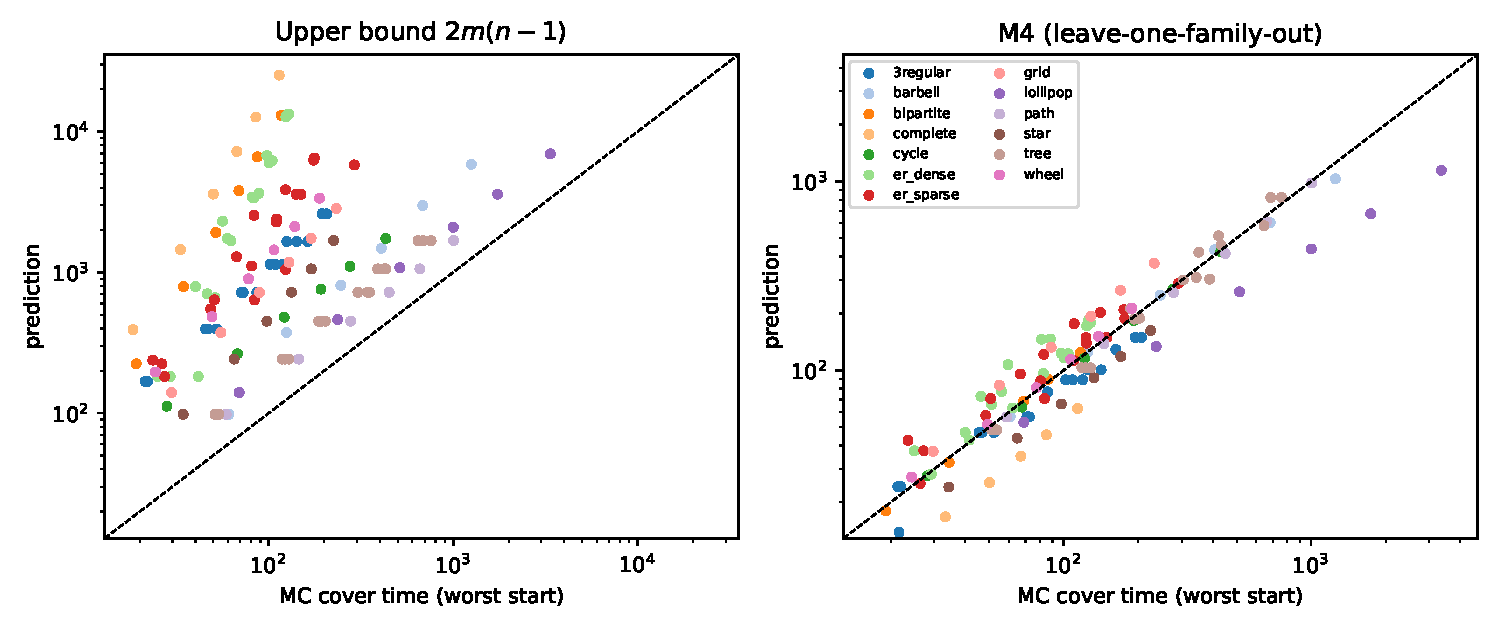
\includegraphics[width=\linewidth]{figs/scatter.pdf}
\vspace{-1.5em}
\caption{Predicted vs.\ Monte Carlo worst-start cover time (log--log). Left: bound $2m(n-1)$. Right: M4 under leave-one-family-out CV. The dashed line is $y=x$.}
\label{fig:scatter}
\end{figure}

\begin{table}[t]
\caption{Per-family geometric-mean ratio predicted/true ($1.00$ = unbiased). Values below 1 are underestimates.}
\label{tab:fam}
\centering\small
\begin{tabular}{lccccc}
\toprule
Family & \#graphs & $2m(n-1)$ & Matthews & M4 5-fold & M4 LOFO \\
\midrule
3regular & 18 & 9.94 & 1.56 & 0.93 & 0.84 \\
barbell & 6 & 3.25 & 2.90 & 0.96 & 0.95 \\
bipartite & 6 & 40.98 & 1.04 & 0.99 & 0.99 \\
complete & 6 & 78.77 & 1.00 & 0.62 & 0.52 \\
cycle & 6 & 3.98 & 1.77 & 0.97 & 0.97 \\
er-dense & 18 & 30.41 & 1.68 & 1.20 & 1.32 \\
er-sparse & 18 & 16.68 & 2.02 & 1.17 & 1.21 \\
grid & 6 & 8.18 & 1.74 & 1.45 & 1.48 \\
lollipop & 6 & 2.05 & 3.29 & 0.64 & 0.48 \\
path & 6 & 1.64 & 2.73 & 0.96 & 0.94 \\
star & 6 & 4.82 & 1.03 & 0.83 & 0.69 \\
tree & 18 & 2.21 & 2.17 & 0.97 & 0.97 \\
wheel & 6 & 12.27 & 1.15 & 1.06 & 1.08 \\
\bottomrule
\end{tabular}
\end{table}

\textbf{Error by graph type (Table~\ref{tab:fam}, Fig.~\ref{fig:fam}).} Under LOFO, M4 is accurate on paths ($0.94$), cycles ($0.97$), trees ($0.97$), barbells ($0.95$), complete bipartite graphs ($0.99$) and wheels ($1.08$); the per-family mean absolute log error is $\le 0.12$ for all six. It fails in two ways. (1) \emph{Underestimation} on lollipops ($0.48$), complete graphs ($0.52$) and stars ($0.69$). For complete graphs and stars, $D\le2$ while $d_{\max}=n-1$, so the model sits at an extrapolated corner of feature space. For lollipops, the cover time is driven by walks that keep falling back into the clique, a mechanism that neither $D$ nor $d_{\max}$ represents. (2) \emph{Overestimation} on grids ($1.48$), dense ER graphs ($1.32$) and sparse ER graphs ($1.21$). These are well-connected graphs whose diameter overstates how hard they are to cover. The bounds show a complementary pattern: $2m(n-1)$ is closest on paths and trees ($1.6$--$2.2\times$) and worst on dense graphs ($30$--$79\times$), while Matthews' bound is nearly exact on complete, star and complete bipartite graphs (ratios $1.00$--$1.04$) and loosest on lollipops, barbells and paths ($2.7$--$3.3\times$).

\begin{figure}[t]
\centering
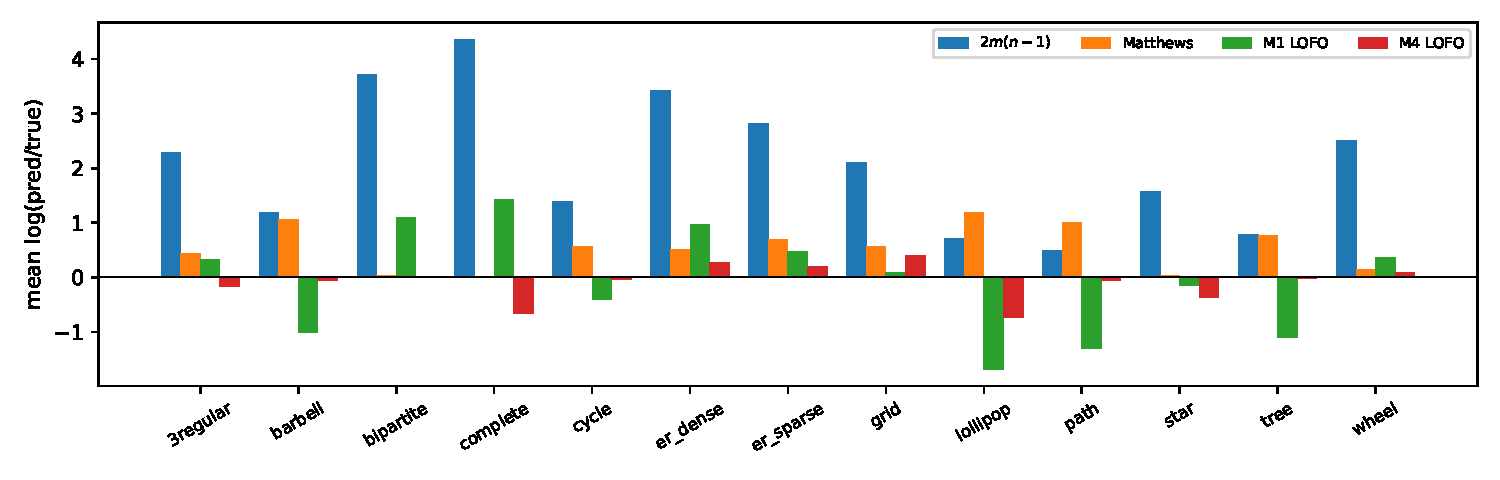
\includegraphics[width=\linewidth]{figs/family_bias.pdf}
\vspace{-1.5em}
\caption{Mean log ratio predicted/true per family (0 = unbiased) for two bounds and two calibrated predictors (LOFO).}
\label{fig:fam}
\end{figure}

\section{Discussion and limitations}
\textbf{Answer to the question.} Yes, on the graphs we tested. Four cheap statistics, effectively three since $m$ is redundant, predict the worst-start cover time of graphs with $n\le30$ to within a typical factor of $1.26$ on unseen families and $1.19$ on unseen graphs from seen families. The bound $2m(n-1)$ is off by a typical factor of about $9$, and Matthews' bound by about $1.8$. The error depends strongly on the graph type: the predictor is reliable on sparse, path-like and moderately symmetric graphs, and off by about $2\times$ on clique-plus-path structures and on the extreme dense or low-diameter corner.

\textbf{Limitations.} (i) \emph{Not a bound}: M4 underestimates about half of the graphs, so it must not replace worst-case guarantees. (ii) \emph{Distribution dependence}: the coefficients reflect our 13 families and six sizes. LOFO estimates transfer to new families, but other families (e.g.\ heavy-tailed or community-structured graphs) may behave differently. (iii) \emph{Small scale}: there are 126 graphs and $n\le30$. We make no claim about asymptotic behaviour, and exponents fitted on a narrow range of $n$ need not extrapolate. (iv) \emph{Target}: we predict the worst-start cover time estimated with a two-stage start selection. On paths the selection loses at most 4\%; we did not verify it exactly on non-symmetric random graphs, where the estimate is a lower bound on the true worst start up to MC noise. (v) Only linear models in log space were tried; per-family failures suggest adding a ``bottleneck'' feature (e.g.\ size of the largest clique attached to a long path), which we leave for future work. This was a deliberately small study, so no hyperparameter search or large sweep was performed.

\textbf{Reproducibility.} \texttt{python code/cover.py} (Python 3.11, NumPy 2.4, NetworkX 3.6; master seed 2026) regenerates all numbers, tables and figures in about 30\,s on a 40-core CPU.

\bibliography{refs}
\bibliographystyle{iclr2026_conference}
\end{document}
